\chapter{Design and Development}\label{chap:design_and_development}
This chapter gives an in-depth look at how the implementation of the code generation tool works, and how it fits together with the DPF Editor and the Xpand framework. The different components and their function will be explained. In the end of the chapter there will be an overview of what has been achieved throughout the development, and what the tool's shortcomings are.

In the Xpand documentation, the mapping between a DSML and the Xpand types are referred to as the metamodel. Hence we will use \emph{metamodel} when describing the \emph{DPF Xpand type mapping}. When referring to the Ecore metamodel in which DPF is specified, we will describe it as \emph{DPF Ecore metamodel}. 

\section{Development Process}
\subsubsection{Development Methodology}
This project has chosen to use \emph{Agile} development methodologies. The methodology chosen for this project is Extreme Programming (XP), although following it completely by the book has not been possible. XP was created by Kent Beck~\cite{Beck:2004:EPE:1076267} which is one of the pioneers in the Agile movement~\cite{agile_alliance}. The reason for choosing XP over other agile methodologies is that it is tought in the MOD251 class at Bergen University College. There are a few constraints which hindered following XP properly; the project had no clearly defined requirements, lack of time and no one else working on the same problem (pair-programming).

In the development phase of the project, the aim was to deliver working software every two weeks coinciding with DPF project meetings. The meetings gave a chance to review what had been done, and the focus area for the next iteration.
  
% Even though some of the 
% \begin{itemize}
%   \item Methodology
%   \item Infrastructure, trac
%   \item No tdd, time
%   \item Learning project. Ingen visste noko om verktøy og korleis ting skulle sjå ut. Difor vanskelig med klar prosess.
% \end{itemize}
\subsubsection{Coding Convention}
XP dictates that one should use a predefined coding convention before starting the development. Such standards aim to result in code that is consistent from developer to developer. It defines how the code looks, but can also include guidelines on which patterns to use and avoid. Although this project was developed by one developer, it needs to be maintained by someone else in the future.
   
The code convention used in this project is Eclipse Naming Conventions~\cite{eclipse_naming_conventions_web}. This convention defines how Eclipse specific elements should be named (e.g. plug-ins and package names). The code convention in general uses Oracle's own guidelines~\cite{java_naming_conventions_web}. The reason for choosing these conventions are that the DPF Editor itself uses them throughout, as well as beeing de-facto standard in the Java ecosystem. Having a completely consistent codebase will improve readability and thus make it easier for new project participants to get started.
  
\subsubsection{Tools}
The development process has been aided by different tools to create an environment which enhances productivity and provides structure. An important tool, even when programming alone, is a bug tracker. Using a bug tracker helps structuring ideas, as well as keeping track of defects. The tool chosen for this task was Trac~\cite{trac}, a lightweight Python based bug tracker with wiki functionality, integration with version control systems (VCS) and the possibility of creating milestones from feature requests and bugs. Along with Trac, Mercurial~\cite{mercurial} was chosen as the VCS. 

The development process was aided by the Eclipse Modeling Tools (Eclipse Java Development Tools with modelling components), using the latest version \emph{Indigo} (3.7)~\cite{Eclipse}. The metamodel is based on the latest released Xpand SDK (1.1.1) which can be found in the modelling components installer inside Eclipse. Logging is used throughout the project for debugging purposes. The logging facility used is called Apache Log4j~\cite{l4j}.

\section{Project Overview}
\subsubsection{Naming Components}
This project uses the same naming conventions which the DPF Editor code base uses. This means all packages starts with \codeText{no.hib.dpf} to denote it is a part of the DPF project. As the sub-project name, \codeText{codegen} is chosen. In time there might be other code generation solutions based on other frameworks than Xpand, and it is suitable to put such projects under the same name. Furthermore, as a component name, \codeText{xpand} is chosen. This is to denote that the particular solution is based on Xpand. \codeText{metamodel} is chosen as sub-component name following the convention used in the Xpand project.
  
The following plug-in projects are defined:
\begin{description}
  \item[\codeText{no.hib.dpf.codegen.xpand.metamodel}]
  \item[\codeText{no.hib.dpf.codegen.xpand.metamodel.test}]
  \item[\codeText{no.hib.dpf.codegen.xpand.metamodel.ui}]
\end{description}
    
% Figure~\ref{fig:dpf_workbench_overview} shows the current architecture of the tools in the DPF Editor, included the code generation component described in this chapter (denoted Xpand and Xpand Extensions).
% 
% \begin{figure}[htpb]
%   \centering
%   \centerline{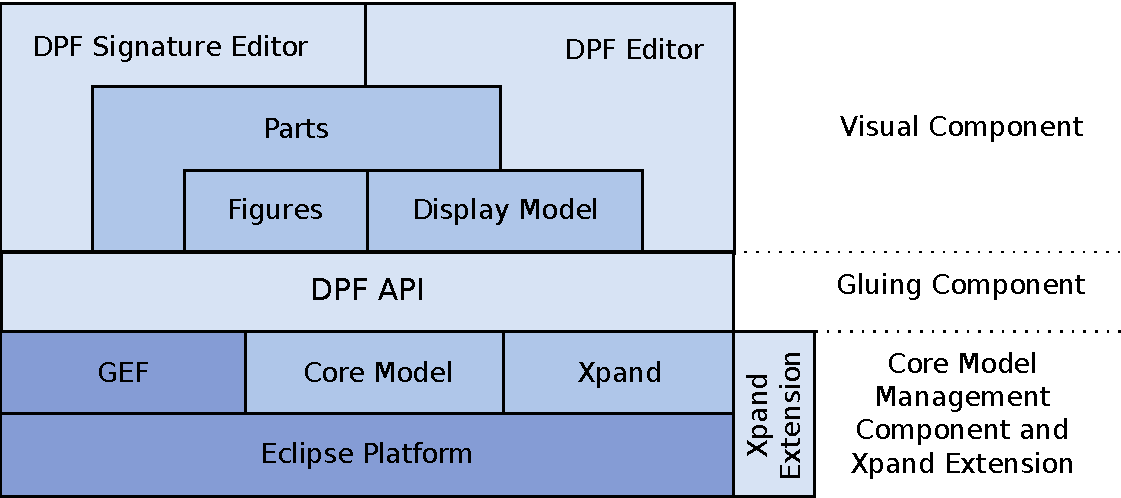
\includegraphics[scale=0.5]{images/component_architechture_r.pdf}}
%   \caption[DPF Editor Architecture]{Architecture of the DPF Editor.}
%   \label{fig:dpf_workbench_overview}
% \end{figure}
% 
% Kodegenerering pluggable component

\section{Problem Description}\label{sec:problem_description}
As discussed in section \ref{sec:metamodels_and_cg}, the DPF Editor is in need for a general solution to creating code generators. Using regular template engines will result in a code generator that would not convey the domain concepts of a DSML. An ideal solution would have the following traits:
\begin{description}
  \item[Clear expression of domain concepts] \hfill \\
  The concepts of the DSML should form the basis for the constructs used in creating templates.
  \item[Integration with Eclipse] \hfill \\
  Editor support is an important feature which makes the template creation process more user-friendly and intuitive. Features like template debugging and profiling are features which also improves the user experience with the tool.
  \item[Standalone generator] \hfill \\
  A generator which does not have to many dependencies are more portable and reusable. With dependencies directly on Eclipse, one would make the solution hard to use in other contexts.
\end{description}

These goals are more or less already achieved in Acceleo and Xpand, but only for the predefined model types which are EMF, UML2 and XSD. This chapter will describe a solution that facilitates the use of DPF models in a custom Xpand metamodel.

\lstset{caption=An example of a Xpand template using the DPF Ecore metamodel as basis.,label=list:xpand_domainconcept,captionpos=b}
\begin{table}[ht]
  \centering
\begin{lstlisting}[showstringspaces=false]
«DEFINE gettersAndSetters FOR core::Node»
	«IF this.getTypeName() != "DomainClass"»
		public «this.getTypeName()» «getter(this)»() {
			return «this.name.toFirstLower()»;
		}
	«ELSE»
		public «this.name.toFirstUpper()» «getter(this)»() {
			return «this.name.toFirstLower()»;
		}
	«ENDIF»
«ENDDEFINE»
\end{lstlisting}
\end{table}

Listing~\ref{list:xpand_domainconcept} shows an example where we use the DPF Ecore metamodel with the EMF metamodel. For each \codeText{DEFINE} block in the templates we need to iterate over \emph{all} nodes of the DPF model, and not the particular collection of nodes conforming to a metatype. This example shows the creation of Java \emph{get} methods from a DSML which contains a \codeText{DomainClass} entity. What we want to achieve is a \codeText{DEFINE} block where we iterate over \emph{only} the nodes that conforms to the \codeText{DomainClass} metatype.

\section{Metamodels in Xpand}
The introduction of this chapter mentions that metamodels in Xpand are a mapping from types in an actual model language (like Ecore) to the Xpand type system. This naming is somewhat confusing, but one can think of it as a metamodel for Xpand's understanding of a model. The metamodel dictates how the input model should be mapped to the Xpand type system, and what kind of mapping this is.

As stated in section \ref{sec:xpand}, Xpand supports a number of predefined metamodels, namely UML2, EMF, XSD and Java beans. Besides these, we have the built-in Xpand types which also can be regarded as a metamodel. In a MWE workflow (from now referred to as workflow, see~\ref{subsub:workflow}) one can take advantage of multiple metamodels at the same time, making each metamodel handle different aspects of the model. 

An important note is that the order of the metamodels is crucial. As an example we can define a workflow which uses three different metamodels (from the Xpand documentation~\cite{xpand}): 
Let us assume that our model element is an instance of the Java type org.eclipse.emf.ecore.EObject and it is a dynamic instance of an EMF EClass Car.
\begin{itemize}
  \item Built-in metamodel (always first)
  \item Java beans metamodel
  \item EMF metamodel
\end{itemize}
If we want to match \codeText{Car} against \codeText{EObject} in the EMF metamodel we bump into a problem: the first match we get is from the built-in metamodel where we get the Xpand type \codeText{Object}. This is now our \emph{best-fit} as every metatype has to extend \codeText{Object}. We then proceed to the Java beans metamodel which will return a \codeText{org::eclipse::emf::ecore::EObject} which is a specialized version of \codeText{Object}. The EMF metamodel would have returned \emph{Car}, but was unable as we got a match before the metamodel was queried. This example illustrates how important the proper order of metamodels is. If we had changed the order of the Java beans metamodel and EMF metamodel, the proper value would have been resolved. Note that using e.g. a UML2 and EMF metamodel to handle different parts of a model is a rare scenario. The example shown is relevant because most metamodels take advantage of the JavaBeans metamodel to provide functionality in a Java class without the need for any hand coding.

Figure~\ref{fig:xpand_overview} shows how Xpand works in principle. The figure shows how the DSML initializes one or more metamodels which creates custom Xpand types (henceforth referred to as types). More specifically, the DSML are \emph{interpreted} at runtime by Xpand and mapped to types defined in the metamodel. When the workflow is executed, Xpand will parse and validate the templates, this is done with the help from the metamodel which decides which types should be applicable where. When the code generation phase starts, Xpand will match a defined input model against the template. This is done through calls against the metamodel as well.

\begin{figure}[h]
  \centering
  \centerline{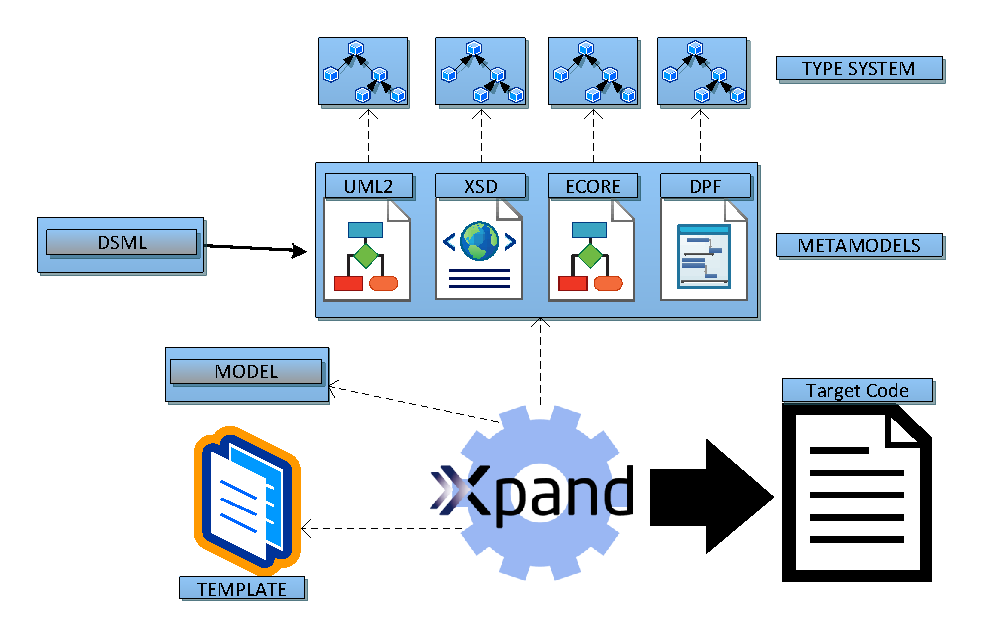
\includegraphics[scale=0.7]{images/xpand.pdf}}
  \caption[Xpand metamodels]{Figure shows how the Xpand metamodels work.}
  \label{fig:xpand_overview}
\end{figure}

A metamodel in Xpand must implement the \codeText{MetaModel} interface. The most important methods that needs implementing are the following:
\begin{description}
  \item[\codeText{getKnownTypes()}] Returns a set of types which represents all of the types the system know of.
  \item[\codeText{getType(Object type)}] Returns a corresponding type which the parameter object is matched against. The objects which is matched against \codeText{getType} are the model objects from either the DSML or instance model. We have to check the object's DPF type to decide how to handle it using the Java operator \codeText{instanceof}.
  \item[\codeText{getTypeForName(String typeName)}] When processing a template, there are type identifiers in the different statements. An example of this is:
  \begin{plainlisting}
«DEFINE test FOR my::namespace::StateType»
  \end{plainlisting}
  The type identifier \codeText{my::namespace::StateType} would be queried against the metamodel to retrieve its designated type, or create a new type if it do not exist.
  \item[\codeText{getNamespaces()}] Returns a set of strings which defines what namespaces the metamodel should handle.
\end{description}

% - figur som viser modell -> interpreter -> conforms til metamodell (vis alle typar) -> lagar typar... conceptual model
% - figur som viser DPF model/metamodel -> DPF Xpand metamodel (Vis internal mm og internal m) -> types?
% -
\subsection{The Xpand Type System}\label{sub:type_system}
The purpose of the type system is to create a common representation of the input models, which can be used as a basis for creating tooling. I.e. rather than creating specialized solutions for a particular model type, we have a general "model" to adhere to. Creating types is also a way to extend the existing functionality in a model; the type system is a \emph{reflection}\footnote{Reflection is the process of dynamically load classes and functionality at runtime.~\cite{reflection_tutorial}} layer which can be extended with the implementation of metamodels. A type in Xpand contains a name, properties and operations, as well as information about inheritance. The type system in Xpand provides access to types based on the metamodels which are used.

Names have the option of using namespaces, which are delimited using "::". In the EMF metamodel, the package name(s) in a model is used as the namespace(s). E.g. with the DPF Ecore metamodel one would have \codeText{no::hib::dpf::core} as the namespace prefix to a type. When using these types in the templates one can import the namespace so that the namespace prefix can be omitted.

When creating a metamodel for Xpand, the types may contain primitives, like string, integer or floats. These types can be wrapped in a tailored solution, e.g. creating a type for floats with operations focused on a particular domain like finance. Often the existing functionality is the best fit to handle primitives as Xpand contains additional functionality for the primitives string, boolean, real and integer. The string class in particular provides methods that is useful in a code generation context, like the "+" operator for string concatenation, regular expressions and more. In addition to the primitives, Xpand has defined a few collection types: Collection, List and Set which corresponds to their Java counterpart (\codeText{java.util.*}). To implement a general approach for the collection types, Xpand uses the concept of \emph{parameterized types}\footnote{A parameterized type in Xpand is a type which has an inner type. The inner type defines what type a collection can contain and must be a Xpand type.}.

As mentioned a Xpand type contains properties and operations based on reflection. Along with static properties, they are what is called \emph{features}. 
\newpage
The features are defined as following:
\begin{description}
  \item[Attribute] \hfill \\
  An attribute contains a name and a return value which is another type.
  \item[Operation] \hfill \\
  An operation is structurally identical to Attributes with the addition of parameters.
  \item[Static Property] \hfill \\
  A static property provides the same functionality as enums or constants. It has no parameters.
\end{description}

In Ecore, every attribute can have a specified type (like \codeText{EString}), and the \codeText{EClasses} can inherit a super-type. When mapping types which have its foundation in a Java class, we can take advantage of the JavaBeans metamodel for providing the functionality it contains. Instead of defining the JavaBeans metamodel within the workflow, it is possible to use it directly in our own metamodel. E.g. the EMF metamodel relies on the JavaBeans metamodel for handling types which is external to the Ecore model.

\section{DPF Xpand Metamodel}
As the problem description (\ref{sec:problem_description}) suggests, using the DPF Ecore with the Xpand EMF metamodel will result in a tedious and unintuitive solution that does not convey the domain concepts of a DSML. As the predefined metamodels do, the DPF metamodel must implement the \codeText{MetaModel} interface. The DPF metamodel behaves like any other metamodel, and can be used in the same manner. Although not properly tested, the metamodel should work seamlessly with all of the predefined components in Xpand.

\subsection{Considered Approaches}\label{subsec:considered_approaches}
Before initiating the work on creating a Xpand metamodel, a different approach was considered due to the high learning curve of Xpand's internals. Since EMF is supported "out of the box", the first thought was to create a model-to-model transformation from DPF to EMF. This approach is valid, but as we discussed in section \ref{sec:xpand} it would restrict the functionality provided to what was defined in the EMF metamodel. A model-to-model transformation from DPF to EMF is probably work worth a master's thesis by itself, and was thus not considered to be a viable solution. 

Another approach considered (see figure~\ref{fig:xpand_dpf_m2m}) was a simplified model-to-model transformation where an Ecore model was built programmatically from a DPF specification focusing on the basic constructs like nodes and arrows. To make this work, we would have to create an (dynamic) Ecore model on the fly and generate a .ecore file which would provide editor support. To make things worse, dynamic EMF does not support creating custom operations like regular EMF does. The biggest problem with this approach however, is that the operations which would be provided through Xpand, would be the generic EMF API. This means we would be back to comparing \codeText{EClass} entities with their name to find a specific DSML node and thus provide no benefit at all.

\begin{figure}[htpb]
  \centering
  \centerline{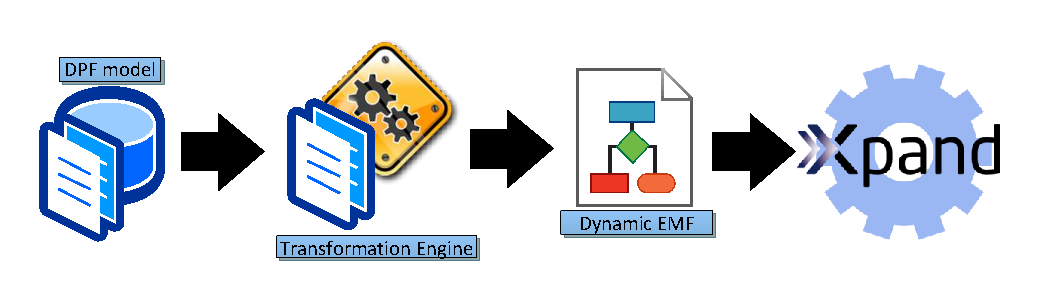
\includegraphics[scale=0.8]{images/dpf_to_emf.pdf}}
  \caption[Model-to-model tranformation from DPF to EMF]{Figure shows the idea behind one of the considered solutions.}
  \label{fig:xpand_dpf_m2m}
\end{figure}

% m2m->emf->xpand->output figur?

\subsection{Packages}
The basic structure of the \codeText{no.hib.dpf.codegen.xpand.metamodel} project contains four different packages.
\begin{description}
  \item[no.hib.dpf.codegen.xpand.metamodel] \hfill \\
  Contains the metamodel class which perform and store all the mappings towards our custom types. It also contains an interface which defines the names of the entities in DPF (e.g. Node, Constraint, Arrow etc.).
  \item[no.hib.dpf.codegen.xpand.metamodel.typesystem] \hfill \\
  The type system package contains utility functionality which are used by the type classes and other parts of the system.
  \item[no.hib.dpf.codegen.xpand.metamodel.typesystem.types] \hfill \\
  This subpackage contains classes for all the custom types. This package is internal, and is not exposed to other plug-ins.
  \item[no.hib.dpf.codegen.xpand.metamodel.workflow] \hfill \\
  This package contains the workflow component \codeText{DpfReader} which handles the initialization of the metamodel, i.e. it loads the DSML's and the model's specification.
\end{description}

\subsection{Structure of the Metamodel}
A way of looking at the metamodel is a black box where you insert the DSML and its instance, and are then able to query it with objects or names which then returns a corresponding type.

\begin{figure}[htpb]
  \centering
  \centerline{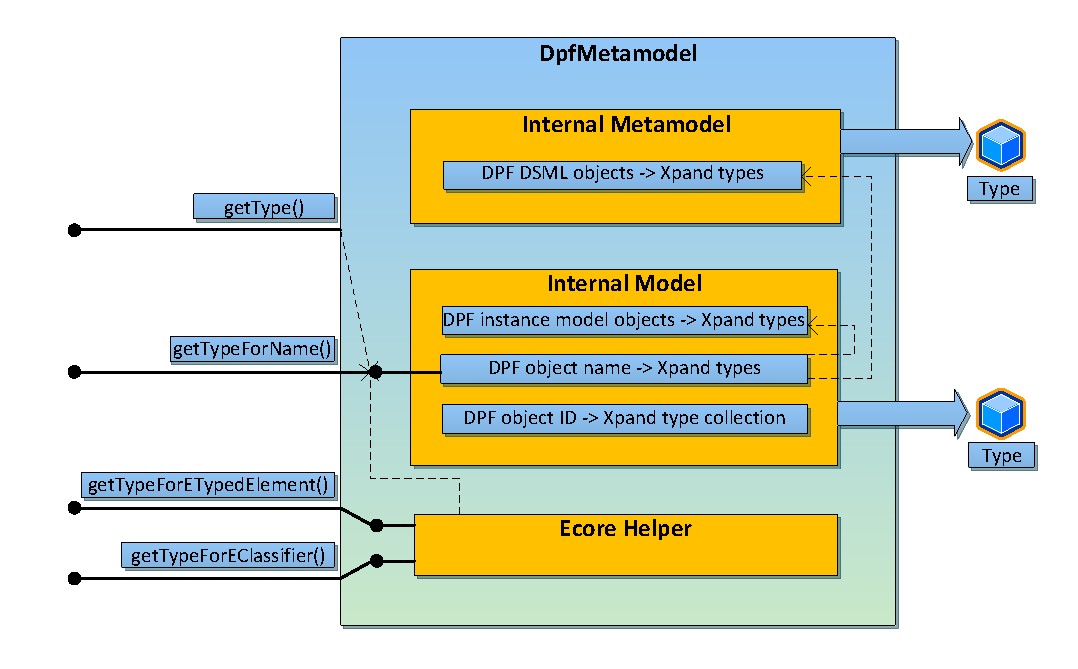
\includegraphics[scale=0.8]{images/metamodelcomponent.pdf}}
  \caption[View of the structure of the metamodel]{Figure shows the internals of a DPF metamodel.}
  \label{fig:metamodel_component}
\end{figure}

The metamodel class has three internal classes with their own responsibility. Figure~\ref{fig:metamodel_component} shows a \emph{internal metamodel}, an \emph{internal model} and what is called the \emph{Ecore helper}. The predefined metamodels in Xpand usually match an object to its metaobject and return that, but in DPF we have a lot of idiosyncrasies which makes it easier to have a representation of the model as well. An important observation is that every call to the metamodel will ultimately go through \codeText{getTypeForName}, and return a result from the internal metamodel \emph{or} the internal model.

There is no validation of the models implemented in the metamodel. The DPF Editor enforce the consistency and validity of the DSML's typing through checking for graph homomorphisms~\cite{Bech11}. Even though we reflect both the DSML and instance model in the metamodel, we do not check for graph homomorphisms between them. When a DSML or instance model is used within the metamodel it is assumed to be valid, both concerning constraints and typing.

\subsubsection{Internal Metamodel}
The internal metamodel represents the DPF DSML and its concepts. When the method \codeText{addDpfMetaModel(Specification)} is called, the \codeText{Specification} object representing the DSML is iterated over, and each DPF type gets matched through a map structure called \codeText{metaModelCache}. This particular mapping is mapped with the DPF model objects from the DSML as keys, and a corresponding type as value. If the type does not exist, a new one will be created with the DSML entity's name as name. In addition to the DSML types, we add two "dummy types", namely \codeText{Node} and \codeText{Arrow} for reasons explained in the next section. Each DSML entity gets stored with its namespace prefixed, although it is hardcoded for DPF models at this point (see~\ref{subsub:namespaces}).
\begin{figure}[h]
  \centering
  \centerline{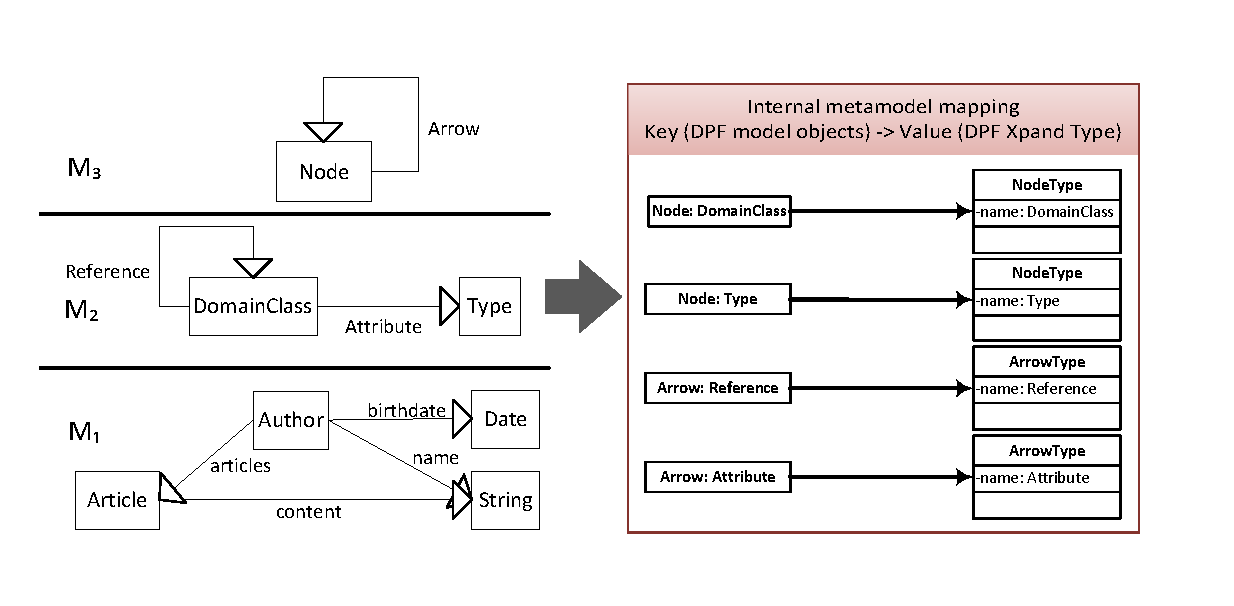
\includegraphics[scale=0.8]{images/dpf_to_type_mapping.pdf}}
  \caption[Mapping from DPF types to DPF Xpand metamodel types]{Figure shows a simple mapping between a DSML and Xpand types.}
  \label{fig:dpf_to_type_mapping}
\end{figure}

Figure~\ref{fig:dpf_to_type_mapping} shows how a simple DSML is mapped to corresponding types within the type system. 

\subsubsection{Internal Model}
An internal model represents the DPF instance model of the DSML. This class is initiated when \codeText{addDpfModel(Specification)} is called. As with the internal metamodel, we create a object to type mapping, but this time with the instance DPF specification as the basis. The reason for mapping the instance model is that we need to retrieve the correct object when traversing the graph. When chaining method calls, we would have returned the DSMLs objects rather than the instance, thus looking up the wrong objects in the metamodel.

Next we create a DPF type ID\footnote{Each node, arrow, constraint and graph has a unique id within the \codeText{Specification} object.} to list of DPF objects mapping. The list of objects is built using all the objects in the instance model which has the same metatype (ID). This is not necessary, but retrieving all instances of a DSML type is a common operation, and a collection simplifies that process. 

The last and most important mapping is the type name to type mapping, which is used for resolving every query to the metamodel. This mapping points to both the internal metamodel mapping \emph{and} the internal model's DPF object to type mapping. As figure~\ref{fig:metamodel_component} shows, the Ecore helper also uses the name to type mapping. Using names to identify objects is unfortunate due to its ambiguity, but necessary as all type definitions in the templates are simple names. An example issue is when nodes and arrows, or more than one node or arrow has the same name: which type is the correct one? The only way to deal with this is to check if the object retrieved from a mapping corresponds with what is queried. The type names are stored with their respective namespace prefix.

\subsubsection{Ecore Helper}
For convenience purposes we take advantage of the functionality specified in the DPF Ecore metamodel. From the types created for the metamodel this helper class gets called to resolve attributes and operations on the \codeText{EClass} in which any DSML/model type is an instance of. It is very useful to get operations like \codeText{get/setName} or \codeText{get/setGraph} for "free", i.e. without having to define them manually in the types. The names of getters are shortened to "name" instead of "getName" for convenience.

\subsection{Type System}\label{subsec:type_system}
The types created for our metamodel reflects the types which DPF defines. The purpose of the types is to encapsulate the model object and expose its functionality through the Xpand type system. As stated in section \ref{sub:type_system} we can also define our own functionality through the Xpand API. This proves to be quite useful, as the DPF API is not tailored for graph traversal and code generation. As an example, we can take outgoing arrows from a node in the DPF Ecore metamodel where the only possibility is to retrieve \emph{all} the outgoing arrows. When writing templates it is convenient to not iterate over \emph{all} the arrows and decide its type within the template itself, as this would create a lot of complexity. A possible solution could be to create an extension that built collections of arrows upon generator execution, but this would be a lot of manual labour and unnecessary because it can be automated. This is where our custom types come to the rescue; we simply define new methods that can be used within the template environment. This particular example problem is tackled by creating a mapping from a DSML type ID to a collection of instance model nodes that has the same metatype ID (see previous section). 

\begin{figure}[htpb]
  \centering
  \centerline{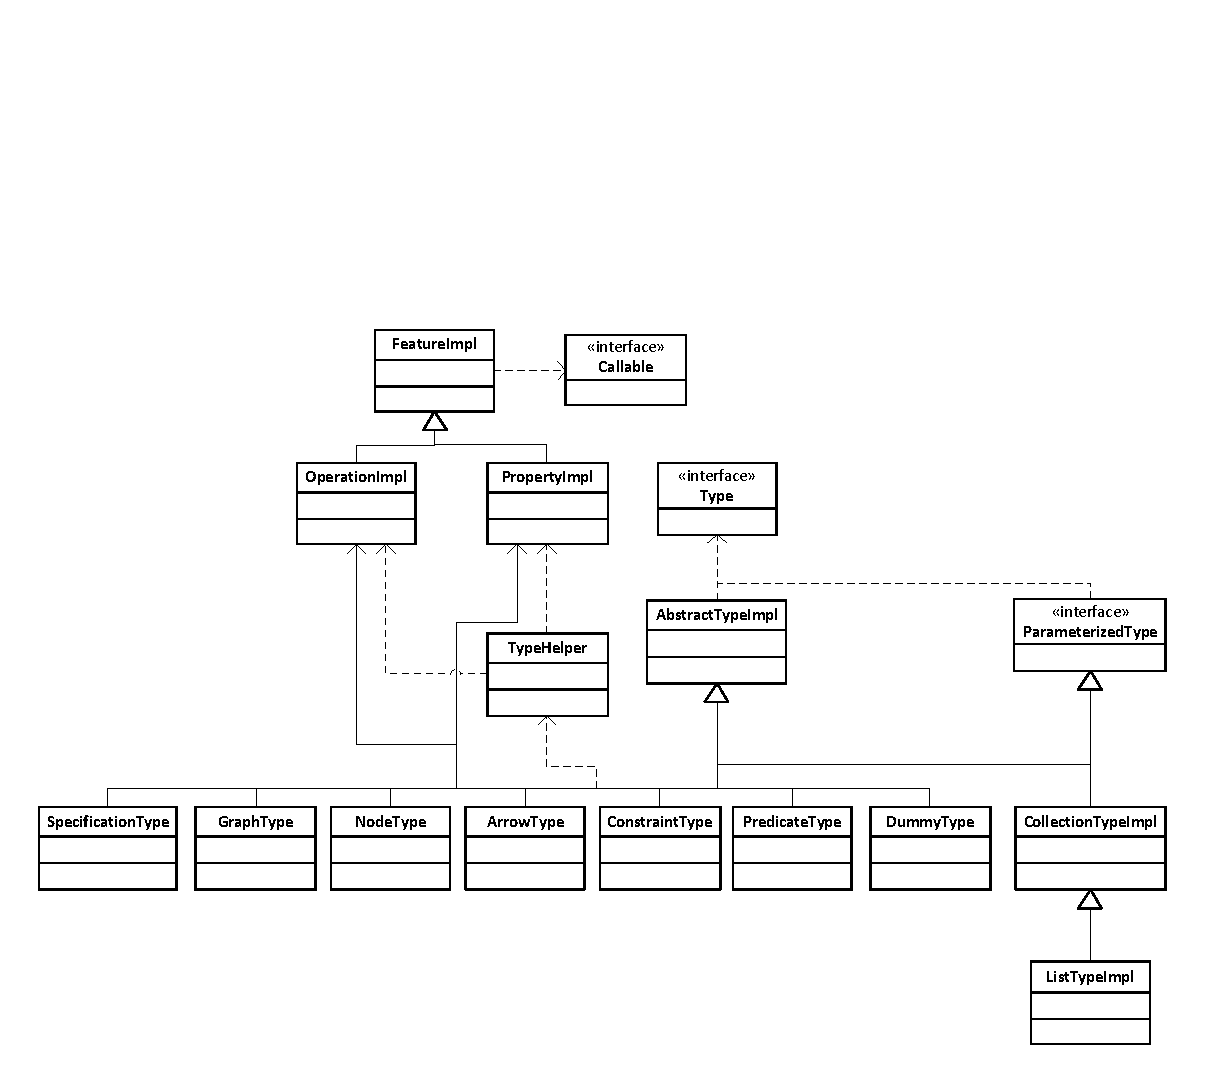
\includegraphics[scale=0.8]{images/typeuml.pdf}}
  \caption[DPF Xpand types]{Figure shows the type system in the DPF Xpand metamodel.}
  \label{fig:xpand_dpf_types}
\end{figure}

Figure~\ref{fig:xpand_dpf_types} shows an overview of the DPF metamodel's typesystem. For each DPF concept, we have a corresponding type. All of the types inherits \codeText{AbstractTypeImpl} which in its turn implements the \codeText{Type} interface. We also see that the \codeText{CollectionTypeImpl} implements the \codeText{ParameterizedType} interface which defines an inner type of the collection, which is how parameterized types are declared in Xpand. As in the \codeText{java.util} package, the list and set is a specialized case of a collection.

We also see that we have referenced attributes, operations and static properties from our types. \codeText{AbstractTypeImpl} does caching of all the \emph{features} within a type automatically. The \codeText{TypeHelper} class is responsible for creating all the Ecore features for each type based on the DPF type. I.e. an instance of \codeText{Arrow} will provide getters and setters for names, retrieving its graph, target and source etc.

Not all of the custom types provide any alterations to their corresponding DPF entity's type. \codeText{ConstraintType}, \codeText{PredicateType} and \codeText{SpecificationType} are only defined through the functionality in the DPF Ecore metamodel. Due to recent API changes there has not been a priority to define custom behaviour as the DPF Ecore functionality is satisfactory.

\begin{figure}[htpb]
  \centering
  \centerline{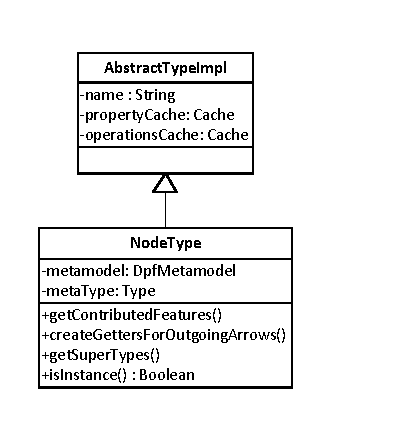
\includegraphics[scale=0.8]{images/nodetypeuml.pdf}}
  \caption[NodeType UML]{A class diagram showing a \codeText{NodeType} and its parent. This graphic only shows selected entities within the classes for simplicity.}
  \label{fig:nodetype}
\end{figure}

Figure~\ref{fig:nodetype} represents a the "anatomy" of a \codeText{NodeType}. All of the specified types for the DPF metamodel inherits \codeText{AbstractTypeImpl}. We see \codeText{AbstractTypeImpl}'s data fields, which contains \codeText{Cache}\footnote{A \codeText{Cache} object is a wrapper around \codeText{java.util.HashMap} with some additional functionality.} objects that store all the \emph{features} of the metamodel. That is, when the method \codeText{getAllFeatures()} is called (which is defined through the Xpand interface \codeText{Type}), the class calls \codeText{getContributedFeatures()} which is an abstract method implemented in the subclass. This is an example of the \emph{template pattern}~\cite{Martin:2003:ASD:515230}.

The Xpand type system supports inheritance within the types. The Java objects which represent the Xpand types has no inheritance in between each other. This inheritance is defined through the method \codeText{getSuperTypes()}, where a type returns a set of Xpand types which the particular type should inherit. In the DPF metamodel each type from the model instance inherits its metatypes's type. Figure~\ref{fig:xpand_dpf_types} shows a type called \codeText{DummyType}, which is a type that only contains its name, no operations and attributes are defined. The reason for implementing this type is to use it as supertypes for the DSML's and instance model's types, for the purpose of defining general methods on e.g. nodes like \codeText{getOutgoingArrows}. Although that particular method is implemented through the DPF Ecore, it will not work due to the DSML and instance model types beeing different from eachother (e.g. a \codeText{NodeType} called \codeText{Process} is not the same type as a \codeText{NodeType} called \codeText{Control}).

The \codeText{createGettersForOutgoingArrows()} is a method which returns custom operations for the node. In short, the method creates a "get" method for each type of arrows which is outgoing from the node. This is the implementation of the scenario mentioned in the beginning of this section.

%dummytype!!!!
% DPF typar som arvar kvarandre
% oversiktsfigur frå nye DPF paper 
% 
% Utfordringar med typar: f.eks Arrow som dummytype, Xpand tek ikkje hand om subtypar.
% Grunn til å bruke model som lag er at ein kan finne kva piler som går kvar når Node.getAttrib()[0].target.Node -> sjekk arrowtype
% \item[\codeText{getType(Object type)}] Returns a corresponding type which the parameter object is matched against. The objects which is matched against \codeText{getType} are the model objects from the DPF \codeText{Specification} object which contains the DSML or model. Every call needs to be handled with the right type in mind because we can not identify the different parts of a DPF model in the same way. 

% typeforname brukt i gettype
\subsection{Reader and Workflow}\label{subsec:reader_workflow}
For the metamodel to work in a MWE workflow, we need a reader component which initates the metamodel with data. In the DPF metamodel's case, we want the reader to load both a DSML and model. A component in Xpand is a class which implements the interface \codeText{WorkflowComponent}. 
% The class consists of a few methods which needs to be implemented

\begin{figure}[htpb]
  \centering
  \centerline{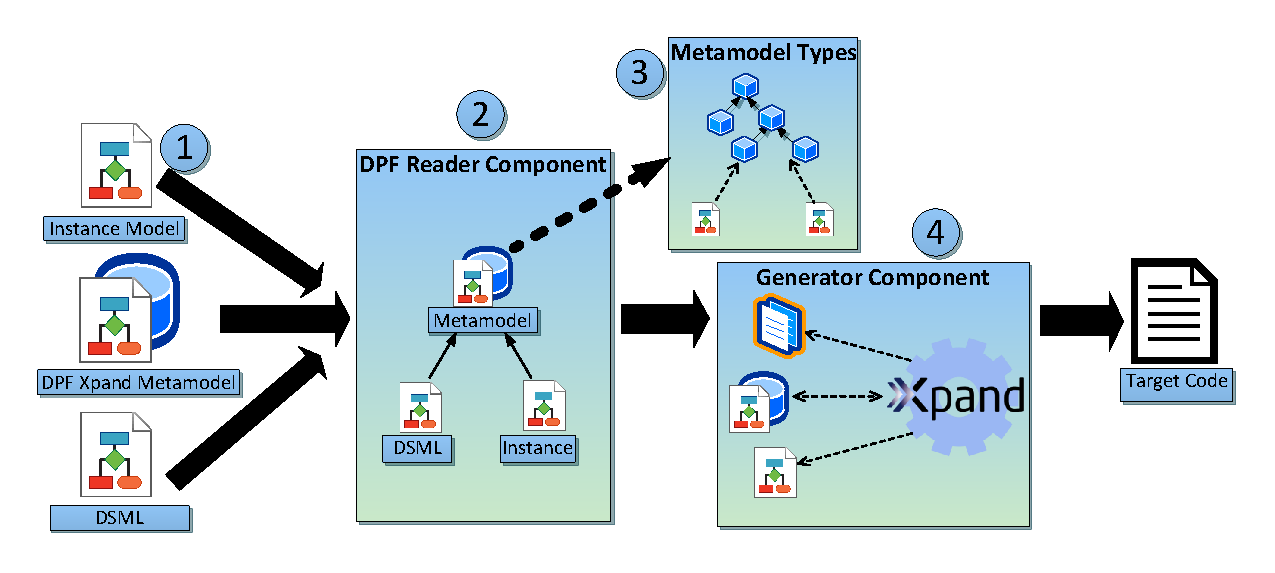
\includegraphics[scale=0.7]{images/xpand2.pdf}}
  \caption[Workflow using the DPF Xpand Metamodel]{Figure shows how the Xpand DPF metamodel works in a workflow.}
  \label{fig:xpand_dpf_workflow}
\end{figure}

Figure~\ref{fig:xpand_dpf_workflow} shows how the workflow proceeds from start to end. This visualization only contains two components, the DPF Reader and the Xpand Generator component.
\begin{enumerate}
  \item The first step in a workflow is to declare properties. We assign a name to e.g. a path or value to simplify the appearance of the workflow file. This is optional as you can use paths directly in the components, the assigned ID is merely an alias. What is important is instantiating the metamodel and assigning it an ID, making it available across components within the workflow. See the three first lines of listing~\ref{list:dpf_component} for example.
  \item The DPF Reader component takes two paths or URIs to the serialized versions of both a DPF DSML and its instance. The purpose of the reader is to initialize the metamodel. The component can be declared more than once with different metamodels and DSMLs.
  \item This step illustrates the mapping from DPF types (from both the DSML and instance model) to Xpand types within the metamodel.
  \item The generator component shows how the Xpand generator utilizes the metamodel by querying it for suitable types based on type definitions in the template, as well as the input model from the reader.
\end{enumerate}

\lstset{language=xml,caption=A MWE workflow that depicts the DPF Reader component.,label=list:dpf_component,captionpos=b}
\begin{table}[ht]
  \centering
\begin{lstlisting}[showstringspaces=false]
<property name="dpf_model" value="/path/to/resource/model.xmi" />
<property name="dpf_metamodel" value="/path/to/resource/metamodel.xmi" />
<bean id="mm_dpf" class="no.hib.dpf.codegen.xpand.metamodel.DpfMetamodel"/>

<component class="no.hib.dpf.codegen.xpand.metamodel.workflow.DpfReader">
  <dpfMetaModel value="${dpf_metamodel}"/>
  <dpfModel value="${dpf_model}" />

  <metaModel idRef="mm_dpf"/>
  <modelSlot value="dpf" />
</component>
\end{lstlisting}
\end{table}

Listing~\ref{list:dpf_component} shows the DPF Reader component with properties declared for clarity. As previously mentioned, the reader component is needed for initializing the metamodel with the data from models. This happens through the \codeText{<dpfMetaModel>} and \codeText{<dpfModel>} tags. The \codeText{<metaModel>} specifies the DPF Xpand metamodel. Internally, we load the specified XMI files with the DPF Core API and call \codeText{addDpfMetaModel} and \codeText{addDpfModel} on the metamodel. The \codeText{<modelSlot>} tag stores the \codeText{Specification} object of the instance model for use in the \codeText{<expand>} statement in the generator component (see listing~\ref{list:workflowexample}).

\newpage
\subsection{Dependencies}
Using a framework like Xpand instead of a simpler solution, often entails some dependencies. The goal of creating a standalone code generation facility is somewhat hard to achieve. If we look past the dependencies of the Xpand framework, the \codeText{no.hib.dpf.codegen.xpand.metamodel} contains a very limited amount of dependencies:
\begin{description}
  \item[no.hib.dpf.core] The DPF core API.
  \item[org.eclipse.emf.mwe.core] Used for the workflow specific code, i.e. the DPF Reader component.
  \item[org.eclipse.xtend] Contains the type system specific functionality.
  \item[org.apache.log4j] The logging facility used for debug statements within the metamodel and its types.
\end{description}

In a language workbench setting, the generators will always be used with the DSML. Using the Xpand framework for the code generation is then not a problem because the dependencies are fulfilled through the language workbench. A scenario could be that one would want to use Xpand without Eclipse; this is possible as Xpand can run standalone.

An interesting scenario could be where you did not want the whole language workbench tooling, but a lightweight textual solution based on e.g. Florian Mantz' textual DPF tool. In such a scenario it could be interesting to generate a code generator for a DSML that takes textual input (instance models) and outputs code. I.e. generate a standalone generator for a particular DSML. This is called a \emph{generator generator}~\cite{tolvanen:dsm}.

\subsection{Testing the Metamodel}\label{subsec:mm_test}
Creating tests for the code generation tool is important, as there is a lot of corner cases that is hard to predict when creating a metamodel. Unfortunately, test-driven development (TDD) was not an option because of time constraints. Another problem is the lack of expert domain knowledge; learning the ins and outs of DPF was not required to create a usable solution. With the adoption of the tool, identifying corner cases will be a lot easier. The most basic tests as loading models into the Xpand metamodel, and retrieving a type based on its name can be achieved using plain JUnit test-cases. When we want to test for a more intricate bug, creating tests programmatically is a lot of manual labour. A solution to this is creating a test fixture that can load models, and expect a particular output from the Xpand framework.

Even if we decide to create a test programmatically we need a model to operate on. Besides beeing time consuming work, this poses a difficult problem which needs to be resolved: migration from one model to another. Every time we see a change in the DPF Ecore metamodel, all models created previously are unusable. What is needed is a migration strategy when these changes occur, so that the model based tests will not break on API change.

\subsection{Documenting the Metamodel}
As a lot of projects in the Eclipse ecosystem, the Xpand framework has limited documentation. There exists a user guide which covers most aspects of the tools, although some are more explained than others. Developer documentation is next to non-existing and the code base is almost without any comments. This makes the learning curve very steep when trying to make sense of how Xpand works. The best bet of getting an explanation for any concept or piece of code is through the Eclipse Community Forums~\cite{eclipse_forums}. The response on the \emph{M2T forum} are excellent, with very helpful representatives from Itemis~\cite{itemis}.

To mitigate the poor existing documentation, the project will be well documented. Hopefully, this project will serve as a foundation for further work, and must thus have as low threshold for learning the code as possible. Besides this report, the final code will be properly commented, with an example implemented (see chapter~\ref{chap:case_study} to demonstrate the tool in use. The metamodel will especially be well commented, as the idea behind it might be hard to grasp when diving into the code base.

%   \begin{itemize}
%     \item considered approaches?
%     \item metamodel, types, reader
%     \item Figure showing flow from workflow to transformation
%     \item Typesystem in Xpand
%     \item Custom types
%     \item Dependencies -> kjøring av generator utan eclipse?
%     \item testing the metamodel
%     \item pakkar med i feature/forklaring av pakkar
%     \item handtering av Ecore metamodell
%     \item migrasjon av modellar
%     \item migrasjon av templates!
%   \end{itemize}
\section{Integration with Eclipse}
An important aspect of the language workbench is the integrated tooling. We want an IDE like experience when defining our generators, with the best possible support and tools for writing templates. Xpand provides rich editor support through the metamodel, but it is not ready for use until we have created a \emph{metamodel contributor}.

\subsection{Packages}
\begin{description}
  \item[no.hib.dpf.codegen.xpand.ui] \hfill \\
  Root package which contains the plug-in activator and \codeText{DpfMetaModelContributor} (see next section). 
  \item[no.hib.dpf.codegen.xpand.ui.nature] \hfill \\
  Contains support for a project nature. A nature is a project-type specific environment, which can be used to load project type specific functionality like a specific editor or a property dialog. There is also support for project specific properties (workspace scope) through a generic get/set property class.
  \item[no.hib.dpf.codegen.xpand.ui.wizards] \hfill \\
  The wizards package provides UI classes for the project creation wizard. It also contains a XML parser which parses the workflow XML files and gives the option to alter attributes.
\end{description}

\subsection{Editor Support}\label{subsec:editor_support}
Editor support for metamodels are not quite supported out of the box. The \codeText{MetamodelContributor} interface needs to be implemented and then registered through an \emph{extension point}\footnote{An extension point is provided by a plug-in for enabling other plug-ins to contribute functionality.} within Xpand. The metamodel contributor has one objective; return the DSMLs which should be associated with the editor. The editor support in Xpand provides syntax checking and a dynamic code assistance which provides auto completion and suggestions when writing templates.

\begin{figure}[ht]
  \centering
  \centerline{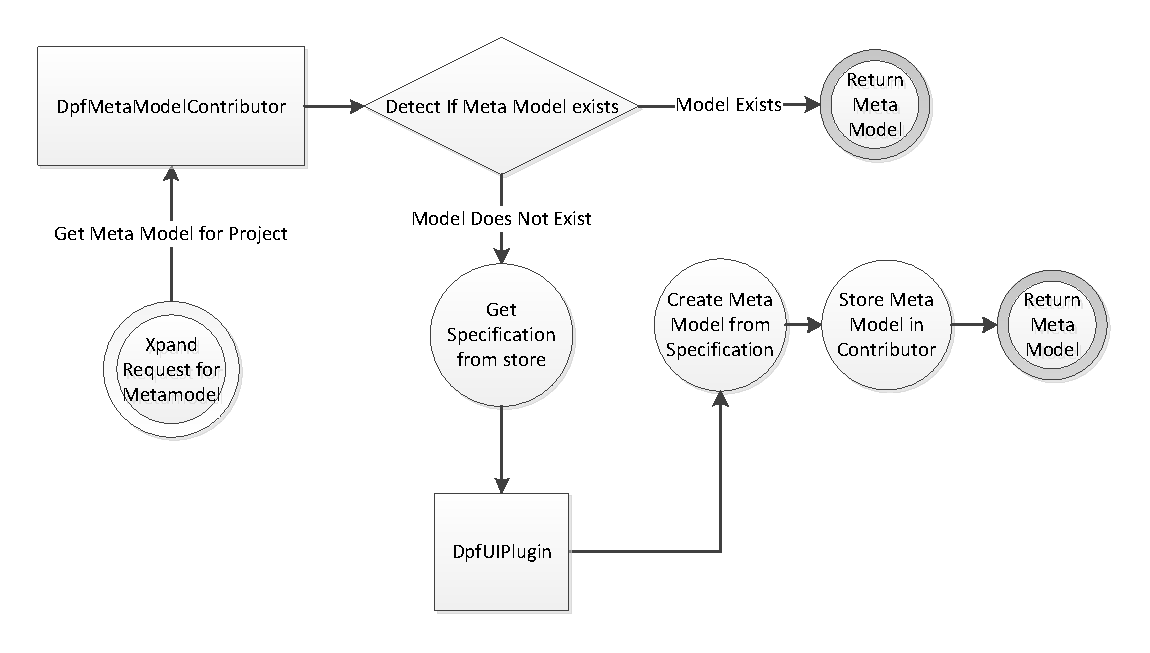
\includegraphics[scale=0.7]{images/metamodel_contributor.pdf}}
  \caption[MetamodelContributor flow chart]{Figure shows the process of retrieving a metamodel for a project.}
  \label{fig:metamodel_contributor_flow}
\end{figure}

Figure~\ref{fig:metamodel_contributor_flow} describes the process of retrieving a metamodel. Xpand will request a metamodel for a project, in which the metamodel contributor will try to look up if it has a metamodel associated with the requested project or not. If not, the metamodel contributor will request that the \codeText{DpfResourceDeltaVisitor} scans the workspace to retrieve any specifications found in either a .prefs file, or a workflow file. The specification found will then be loaded using EMF, and returned to the metamodel contributor where a metamodel object is created with the returned specification as argument. The metamodel contributor then stores the metamodel with the requested project associated for later use and returns the metamodel.

The Eclipse integration and the Xpand generator component both rely heavily on the DPF metamodel. When creating a new DPF Generator Project we specify the location of our DSML through the wizard or the workflow, which then loads the DSML into a metamodel that is associated with the current project. This metamodel is never used for generating code, but only for providing the DSML concepts and its types to the template editor. When generating code, the metamodel and types are instantiated in the workflow, and only exists until the workflow is finished. The template editor's metamodel never has an instance model associated with it, as it is irrelevant.

\subsection{Project Structure}\label{subsec:project_structure}
For the users convenience, we generate a project structure which is ready for use.  Listing~\ref{list:projectstructure} shows the project structure which is generated for the user. The \codeText{src} and \codeText{src-gen} are source code folders where \codeText{src-gen} will contain any generated code. This path is not hardcoded, and can be customized through the workflow file (see listing~\ref{list:workflowexample}). The project is built on top of a Xpand project. This means the project is an Eclipse plug-in which can be used in the same manner as any other Eclipse plug-in project, and we get all the correct dependencies for a Xpand project through the \codeText{MANIFEST.MF} file. The \codeText{.project} file contains details about the project, such as which natures (see next subsection) are activated. This file is essential to let Eclipse know what kind of project we are dealing with. Lastly the \codeText{.settings} folder contains two preference files which are read when the project is recognized as both an Xpand project, and a DPF Generator project. The files define which metamodel is active on the project and where to find the DSML.

\lstset{caption=Listing shows the generated project structure for a DPF Generator Project,label=list:projectstructure,captionpos=b}
\begin{table}[ht]
  \centering
\begin{lstlisting}[showstringspaces=false]
no.hib.dpf.test/
|-- .settings/
|  |-- no.hib.dpf.codegen.xpand.ui.prefs
|  |-- org.eclipse.xtend.shared.ui.prefs                                                                                                                                   
|-- META-INF/
|  |-- MANIFEST.MF
|-- src/
|  |-- template/
|  |   |-- templ.xpt
|  |-- workflow/
|      |-- workflow.mwe
|-- src-gen/
|-- .project
\end{lstlisting}
\end{table}

A template and workflow file are also added. The workflow file contains a simple standard setup, with the DPF Reader component properly defined. The template file contains the "entry" definition of a template, more precisely a \codeText{DEFINE} block for a DPF specification.

\subsection{Project Nature}
In Eclipse the concept of a project nature is to indicate that your project are of a certain type, which uses certain tools. The nature can configure the UI by contributing menu selections, views or any other Eclipse artefact. Natures can also handle project specific properties. 

In the earlier iterations of the codebase, all paths to models was stored in project specific settings. Unfortunately these settings was also workspace specific, which means that if a user checked his project into a VCS and another checked it out, the second user would not have access to the first users settings as to where the models was stored. This problem is avoided by writing a \codeText{.prefs} file in the \codeText{.settings} folder in the project.

This means that the project nature facility in the plug-in is now largely unused, besides always being enabled for new DPF Generator projects. The reason for leaving the code in the plug-in is that it will almost certainly be used in the future if the tool gets further developed.
%   \begin{itemize}
%     \item Plugin and contributor
%     \item Nature?
%     \item Creating project
%     \item Generating project structure with workflow/template <- Illustration
%   \end{itemize}

\section{Shortcomings in the Tool}\label{sec:shortcomings}
\subsubsection{Namespaces and Multiple DSMLs}\label{subsub:namespaces}
In its current state namespaces are not supported. The prefix \codeText{dpf} is hardcoded and used for all types within the metamodel. This poses a problem when one wants to have more than one DSML in the project. It is also not possible to have multiple instance models on one DSML. A solution to this is to run the generator workflow for each DSML and corresponding instance.

This feature was a low priority in this project, and was unfortunately not finished. It might be a usability improvement to manage multiple DSMLs in a single workflow, as well as multiple DSML instances. Multiple DSML instances on a single language requires the implementation of namespaces, as name collisions can occur, and thus returning the wrong node or arrow.

An implementation of this feature is relatively easy. One suggestion is to prefix every entity from the DSML/model with a custom name. Another solution could be to store a map of \codeText{InternalMetamodel}'s and \codeText{InternalModel}'s with the prefix as key.

\subsubsection{Decoupling from \codeText{no.hib.dpf.core}}\label{subsub:decouple}
At this point, there is a very tight coupling between the tool and \codeText{no.hib.dpf.core}. Although a natural dependency, it is problematic that whenever the DPF API is changed, the metamodel might break and its types needs to be updated manually. The nature of the DPF project, where each student works on a separate aspect of the tool, makes it desirable to have each "module" as self sustainable as possible. Learning a new codebase from scratch is a lot of work which can be alleviated by good self-documenting and annotated code, but it is still extra work.

A solution to this problem can be to create an API, beyond the one generated from the DPF Ecore, which is maintained by whoever is responsible for \codeText{no.hib.dpf.core}. Tolvanen and Kelly~\cite{tolvanen:dsm} mentions data-based and message-based APIs to decouple generators from models. A data-based API is basically what we have today, an API which returns parts of the actual model, or a copy. To avoid breaking the API one should mark obsolete methods and classes as \codeText{@Deprecated} rather than removing them. The message-based API is an approach where only proxies for the model are sent back and forth. This means you operate on proxy objects that resolves to a primitive like string or integer at its most basic form.

\subsubsection{Test Coverage}
The current test coverage of the tool is poor. The metamodel and type classes are the only components which have some tests written. The coverage for these components are very limited as well. Besides the lack of time, the issue addressed in section \ref{subsec:mm_test} is the main reason for not creating more tests for the metamodel itself. Other components like the workflow reader and UI related code can be tested programmatically.

\subsubsection{Implementing Constraints and Predicates Using Types}\label{subsub:shortcoming_constr}
When this tool was developed, the signature file (see section~\ref{sec:dpf}) was hardcoded along with its predicates. It was not a priority to do anything about these types, as the Ecore helper within our metamodel exposed the needed functionality. The latest version of DPF Editor gives the opportunity to define custom predicates which opens up new possibilities. There was unfortunately no time to implement this.

Chapter~\ref{chap:case_study} will present a way to simplify the handling of constraints using extensions.

\section{Feature Overview}
We wrap up with an overview of what has been achieved through the development in this project:
\begin{description}
  \item[Xpand metamodel] \hfill \\
  The Xpand metamodel for DPF is the core functionality that lies at the heart of what has been developed in this project. The metamodel is a mapping from the DPF model types to our custom Xpand types. The types exists only in the metamodel, and is available through queries.
  \item[Type system] \hfill \\
  We have defined a type system which Xpand can understand for each of the modelling constructs in DPF. This enables us to easily define new functionality for each modelling constructs, such as DSML specific getters and setters, or utilizing the functionality already defined in the DPF Ecore metamodel.
  \item[Workflow integration] \hfill \\
  With the implementation of the DPF Reader component, we have integrated the metamodel with the Modeling Workflow Engine (MWE). This results in a seamless use of the metamodel between the different components that Xpand offers.
  \item[Eclipse integration] \hfill \\
  With the implementation of a \emph{metamodel contributor}, we can take advantage of all the features which Xpand has to offer. We get editor support for template editing with Xpand, extension editing with Xtend and constraints checking with Check. The editor support contains code completion, syntax coloring, error highlighting, source navigation and refactoring. 
  \item[Project environment] \hfill \\
  As part of the Eclipse integration, we have implemented a project environment that defines a wizard for generating a project structure suitable for code generation. There is also a facilitated a \emph{project nature}.
\end{description}

The time invested in creating this functionality is time well spent, as using any of the alternative approaches (section~\ref{subsec:considered_approaches}) would have been an inferior solution technologically.

Lastly, let us take a look at our problem description in section~\ref{sec:problem_description}. We stated that an ideal solution would solve a few requirements:
\begin{description}
  \item[Clear expression of domain concepts] \hfill \\
  Through the interpreted nature of Xpand, we are able to create an environment for code generation based on the concepts of a DSML rather than an instance model.
  \item[Integration with Eclipse] \hfill \\
  The metamodel and the metamodel contributor give us access to all the features Xpand has to offer.
  \item[Standalone generator] \hfill \\
  This requirement is the one which is not completely fulfilled. A framework with the size of Xpand is bound to have some dependencies. The bright side is that a generator can be executed without Eclipse, with only Xpand, log4j and \codeText{no.hib.dpf.core} as dependencies.
\end{description}
  




